\documentclass[12 pt]{extarticle}

	\usepackage[frenchb]{babel}
	\usepackage[utf8]{inputenc}  
	\usepackage[T1]{fontenc}
	\usepackage{amssymb}
	\usepackage[mathscr]{euscript}
	\usepackage{stmaryrd}
	\usepackage{amsmath}
	\usepackage{tikz}
	\usepackage[all,cmtip]{xy}
	\usepackage{amsthm}
	\usepackage{varioref}
	\usepackage{geometry}
	\geometry{a4paper}
	\usepackage{lmodern}
	\usepackage{hyperref}
	\usepackage{array}
	 \usepackage{fancyhdr}
	 \usepackage{float}
	\pagestyle{fancy}
	\theoremstyle{plain}
	\fancyfoot[C]{\thepage} 
	\fancyhead[L]{Fiche d'exercices}
	\fancyhead[R]{2022-2023}
	
	
	\title{Exercices Chapitre 4}
	\date{}
	\begin{document}

\begin{center}{\Large Chapitre 4 - Proportionnalité}\\
 \end{center} 
\section{Rappels de 4e}
\subsection*{Exercice 1}

Dans les tableaux suivants, reconnaître ceux qui sont des tableaux de proportionnalité. Pour ceux-là, donner le coefficient de proportionnalité. 

\begin{enumerate}
\item $
\begin{array}{|c|c|c|}
\hline
\phantom{000}    12    \phantom{000} 
& \phantom{000}    2   \phantom{000} & 
\phantom{000}
15
\phantom{000}\\
\hline

54 & 9  & 67,5\\
\hline
\end{array}$

\item $
\begin{array}{|c|c|c|}
\hline
\phantom{000}    22   \phantom{000} 
& \phantom{000}   27    \phantom{000} & 
\phantom{000}29
\phantom{000}\\
\hline
2 &7  & 9\\
\hline
\end{array}$

\item $
\begin{array}{|c|c|c|}
\hline
\phantom{000}    20    \phantom{000} 
& \phantom{000}     16  \phantom{000} & 
\phantom{000}
32
\phantom{000}\\
\hline

 15 & 12 & 24 \\
\hline
\end{array}$

\item $
\begin{array}{|c|c|c|}
\hline
\phantom{000}    2    \phantom{000} 
& \phantom{000}     5  \phantom{000} & 
\phantom{000}
7
\phantom{000}\\
\hline

4 & 25 & 49 \\
\hline
\end{array}$

\item $
\begin{array}{|c|c|c|}
\hline
\phantom{000}    10    \phantom{000} 
& \phantom{000}   13    \phantom{000} & 
\phantom{000}16
\phantom{000}\\
\hline
12 &15  & 18\\
\hline
\end{array}$

\item $
\begin{array}{|c|c|c|c|c|}
\hline
\phantom{000}     2   \phantom{000} 
& \phantom{000}    4   \phantom{000} 
& \phantom{000}    8   \phantom{000} 
& \phantom{000}    10 \phantom{000} 
& \phantom{000}   12    \phantom{000}\\
\hline
 7 & 14  &28 & 35 & 42 \\
\hline
\end{array}$

\item $
\begin{array}{|c|c|c|c|c|}
\hline
\phantom{000}    10    \phantom{000} 
& \phantom{000}    13   \phantom{000} 
& \phantom{000}      16 \phantom{000} 
& \phantom{000}      19 \phantom{000} 
& 
\phantom{000}
22
\phantom{000}\\
\hline

20 & 23 & 26& 29&32 \\
\hline
\end{array}$

\item $
\begin{array}{|c|c|c|c|c|}
\hline
\phantom{000}     3   \phantom{000} 
& \phantom{000}    4,5   \phantom{000} 
& \phantom{000}     9  \phantom{000} 
& \phantom{000}      10,5 \phantom{000} 
& 
\phantom{000}
15
\phantom{000}\\
\hline

 7& 10,5 &21 &24,5 & 35\\
\hline
\end{array}$
\end{enumerate}
 
\subsection*{Exercice 2}

Remplir les tableaux de proportionnalité suivants : 

\begin{enumerate}
\item $
\begin{array}{|c|c|c|}
\hline
\phantom{000}     5   \phantom{000} 
& \phantom{000}       \phantom{000} & 
\phantom{000} 25
\phantom{000}\\
\hline
 7 &  84 & \\
\hline
\end{array}$

\item $
\begin{array}{|c|c|c|}
\hline
\phantom{000}    3    \phantom{000} 
& \phantom{000}     5  \phantom{000} & 
\phantom{000}
\phantom{000}\\
\hline
 & 123 & 369 \\
\hline
\end{array}$

\item $
\begin{array}{|c|c|c|}
\hline
\phantom{000}     12   \phantom{000} 
& \phantom{000}   18    \phantom{000} & 
\phantom{000}
30
\phantom{000}\\
\hline
 1696,8&  & 4242 \\
\hline
\end{array}$

\item $
\begin{array}{|c|c|c|c|c|}
\hline
\phantom{000}    7    \phantom{000} 
& \phantom{000}   21    \phantom{000} 
& \phantom{000}   35    \phantom{000} 
& \phantom{000}       \phantom{000} 
& 
\phantom{000}
77
\phantom{000}\\
\hline

 &39  & &104 & \\
\hline
\end{array}$

\item $
\begin{array}{|c|c|c|c|c|}
\hline
\phantom{000}        \phantom{000} 
& \phantom{000}       \phantom{000} 
& \phantom{000}     15  \phantom{000} 
& \phantom{000}      20 \phantom{000} 
& 
\phantom{000}
35
\phantom{000}\\
\hline

 10,2& 15,3 &25,5 & & \\
\hline
\end{array}$

\item $
\begin{array}{|c|c|c|c|c|}
\hline
\phantom{000}     12   \phantom{000} 
& \phantom{000}     32  \phantom{000} 
& \phantom{000}       \phantom{000} 
& \phantom{000}     84  \phantom{000} 
& 
\phantom{000}

\phantom{000}\\
\hline

 2,5 &  & 12,5 & &  25\\
\hline
\end{array}$
\end{enumerate}

\subsection*{Exercice 3}
Un avion réalise un vol Paris-Nice (900 kilomètres) en 1 heure et demie. 
\begin{enumerate}
\item Exprimer sa vitesse moyenne en kilomètres par heure, puis en kilomètres par minute. 
\item Combien de temps faudra-t-il au même avion pour effectuer un Paris-Rome (1100 kilomètres) ? Donner une durée exacte au format \_ heures \_ minutes. 
 
 \item Le même avion met $3$ heures et demie à aller de Paris à Athènes. En déduire la distance entre ces deux villes.  
\end{enumerate}

\section{Pourcentages}
\subsection*{Exercice 4}

Un produit coûte 200 euros. 

\begin{enumerate}
\item Le vendeur propose d'abord une baisse de 10\%. Calculer le prix après cette réduction. 

\item Le prix remonte alors de 10\%. Calculer le nouveau prix, et le comparer au prix initial. 
\end{enumerate}

\subsection*{Exercice 5}

Un produit coûte 100 euros, et augmente de 3\% pendant 5 années consécutives. Calculer ses prix successifs. Exprimer l'augmentation totale en pourcentage du prix initial. 

\subsection*{Exercice 6}

Un produit coûte 10 euros en décembre.
\begin{enumerate}
\item On augmente le prix de 50\% en janvier, puis on revient au prix de départ en février. En mars, le prix baisse de nouveau de $N$\%. Exprimer le prix final en fonction de $N$.
\item Quel doit donc être la valeur de $N$ pour que l'on revienne au prix de départ ? 
\end{enumerate}
 
\subsection*{Exercice 7}

Une personne dépose une somme de $1000$ euros sur un livret à 5\%. (Cela signifie que chaque année, la banque verse 5\% du montant du compte sur celui-ci le 1er janvier).

\begin{enumerate}
\item Exprimer la somme versée sur la banque après la première année. 
\item On suppose que l'on ne rajoute rien sur le compte. Exprimer le montant du livret après $N$ années par une expression en fonction de $N$. 
\item Quel est le montant sur le compte après 15 ans ? 20 ans ? 25 ans ? 30 ans ?

\end{enumerate}

\section{Ratios}

\subsection*{Exercice 8}

Alice, Bob et Charles investissent pour acheter un ticket de loterie à 10 euros. Ils fournissent respectivement 3 euros, 2 euros et 5 euros. 
\begin{enumerate}
\item Quels sont les gains de chacun s'ils gagnent un prix de 700 euros ?
\item Quels sont les gains de chacun si Alice gagne $273$ euros ? 
\item Si Alice gagne $100$ euros de moins que Bob, combien gagne-t-elle ? 
\end{enumerate}


\subsection*{Exercice 9}

Trois personnes misent sur un même numéro. Le premier mise $2$ euros, et le second $3$ euros. 
\begin{enumerate}
\item Les trois joueurs se partagent un gain de $170$ euros, et le deuxième joueur gagne $51$ euros. Combien a misé le troisième joueur ? 
\item S'ils se partagent désormais $360$ euros, combien gagnera le troisième joueur ? 
\end{enumerate}
\subsection*{Exercice 10}

Voici la liste des résolutions standard d'écrans (questions page suivante) : 

\[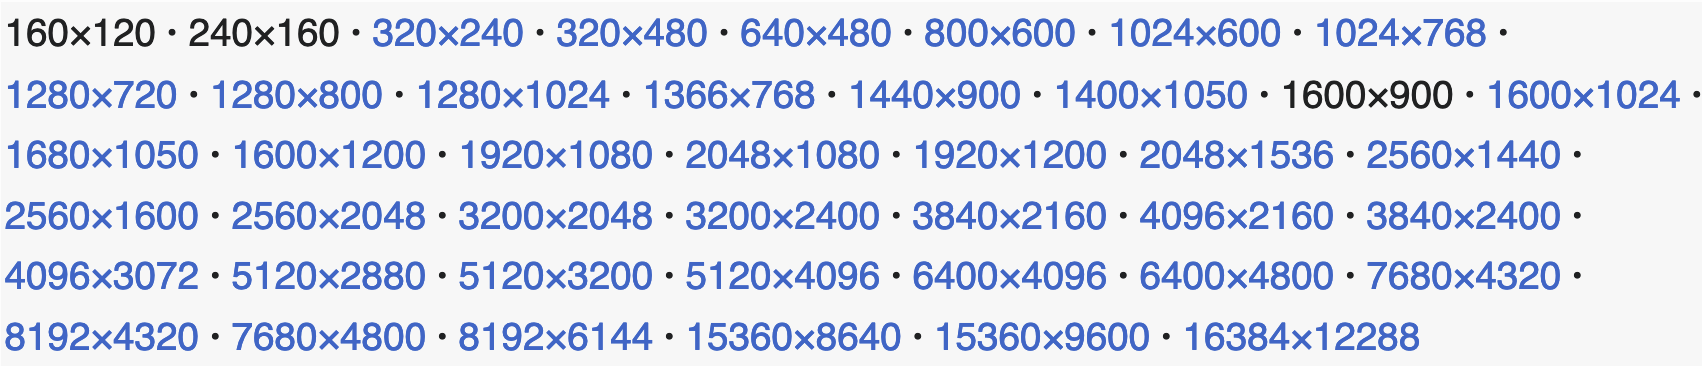
\includegraphics[scale=.5]{Liste.png}
\]

\begin{enumerate}
\item Exprimer chacune de ces résolutions en fonction de leur ratio simplifié largeur:hauteur (on parle également de \emph{rapport de forme}). 
\item Ranger les différents rapports de forme par ordre croissant du rapport largeur/hauteur. 
\end{enumerate}

 	\end{document}
